\section{Sentiment Analysis}
This is the main section as far as the project is concerned, in fact here will be treated the sentiment analysis. It describes the creation of the model and work on the data predicted by the model.
My model can basically be imagined as a function that takes arbitrary text as input, evaluates it, and classifies it into negative and positive.
To develop and train a model with this capability requires many prebuilt datasets of real examples from the Internet. These are then used to feed the model so that it can learn from these datasets and deduce correlations. Based on these correlations, the model will then be able to process arbitrary texts and assign sentiment values to them.

\subsection{The first approach to the thesis}
Before I started doing any work on sentiment analysis, I had to do many hours of research.
At the end of the 5th semester, we saw in class how to do text analysis, so with techniques of:
\begin{itemize}
    \item regex,
    \item sentence segmentation (character sequence into sentences), 
    \item tokenization (character sequence into tokens (words)),
    \item stop word elimination (the, a, to, of, etc),
    \item normalization (U.S.A. or USA as no difference),
    \item lemmatization,
    \item stemming,
    \item using NLTK library.
\end{itemize}

So, the first approach was to work with an NLTK library, and do text analysis.
However, doing research I have seen that in recent times another method has become more famous and has become the state of the art in all respects with regard to the task of text classification, text summarisation, question answering and sentiment analysis.
I am talking about \gls{BERT}.
As I continued in my research I saw not only how famous \gls{BERT} had become in a short time, but also how much it made machine learning work easier, thanks to \gls{BERT}, Natural Language Processing (NLP) became easy and accessible for everyone.
Becoming so used and famous, it caused in a short time the creation of several libraries and methods related to \gls{BERT}.
After working on the datasets, the biggest difficulty was finding the version of \gls{BERT} and related libraries that would best suit them.
For this task, I invested a lot of time and research to figure out which \gls{BERT} is right for me.
Finally, my choice fell on \gls{BERT}-base with \gls{Hugging Face}'s Transformes as library.
The convenience of these transformers is that you can use thousands of pre-trained templates for task text classification, information extraction, question answering, etc. in over 100 languages.

\subsection{Ktrain}
\label{chap:Ktrain model}
Now that I am clear on the tools, all I have to do is set up the work.
To be able to do something of my own I thought to work also on the dataset, so with \gls{Ktrain} I did not use the IMDB dataset, but I opted for the Filmstarts dataset.

\gls{Ktrain} can be used thanks to two different APIs:
\begin{itemize}
    \item automatic API,
    \item manual API.
\end{itemize}

The automatic API has a limited choice of classifiers (6), having to create a model that works on the German language I need a specific classifier, so I am going to use the manual API because I can use any pre-trained model that you can find at the \gls{Hugging Face} website \cite{noauthor_hugging_nodate}.
The manual model is an improvement of the automatic model, the part about the automatic model can be found in \autoref{chap:model filmstars auto}.


\paragraph{Process the data}
The data has been cleaned previously as seen in \autoref{chap:work on dataset}, the data then only needs to be tokenized in order to be used.  


\textbf{What is tokenization?}\cite{noauthor_what_2019}
Tokenization is one of the most common tasks when it comes to working with text data, in a nutshell is the division of a text (sentence, paragraph or a whole text) into individual words . Each word is called a token.
However, \gls{BERT} cannot use words directly, so there will be a need to encode each token into numbers so that it is usable by the machine.
\gls{BERT} only digests tokens with a maximum length of 512.
It does not make sense to use the maximum length when the tokens are shorter, so in order to save model work and to speed up preprocessing work I need to find the maximum length of each review.

What I need to do now is to figure out the maximum length of each review, meaning that I just need to find what is the max\_len I am interested in to create the model:

    \begin{tcolorbox}[breakable, size=fbox, boxrule=1pt, pad at break*=1mm,colback=cellbackground, colframe=cellborder]
\begin{Verbatim}[commandchars=\\\{\},fontsize=\footnotesize]
\PY{n}{textToCheck} \PY{o}{=} \PY{n}{film\PYZus{}review\PYZus{}df}\PY{o}{.}\PY{n}{Review}\PY{p}{[}\PY{l+m+mi}{1}\PY{p}{]}
\end{Verbatim}
\end{tcolorbox}

    \begin{tcolorbox}[breakable, size=fbox, boxrule=1pt, pad at break*=1mm,colback=cellbackground, colframe=cellborder]
\begin{Verbatim}[commandchars=\\\{\},fontsize=\footnotesize]
\PY{k}{for} \PY{n}{txt} \PY{o+ow}{in} \PY{n}{textToCheck}\PY{p}{:}
    \PY{n}{tokens} \PY{o}{=} \PY{n}{tokenizer\PYZus{}hugg}\PY{o}{.}\PY{n}{encode}\PY{p}{(}\PY{n}{txt}\PY{p}{,} \PY{n}{max\PYZus{}length}\PY{o}{=}\PY{l+m+mi}{512}\PY{p}{)}
    \PY{n}{token\PYZus{}lens}\PY{o}{.}\PY{n}{append}\PY{p}{(}\PY{n+nb}{len}\PY{p}{(}\PY{n}{tokens}\PY{p}{)}\PY{p}{)}
\end{Verbatim}
\end{tcolorbox}

\begin{figure}[ht!]
\centering
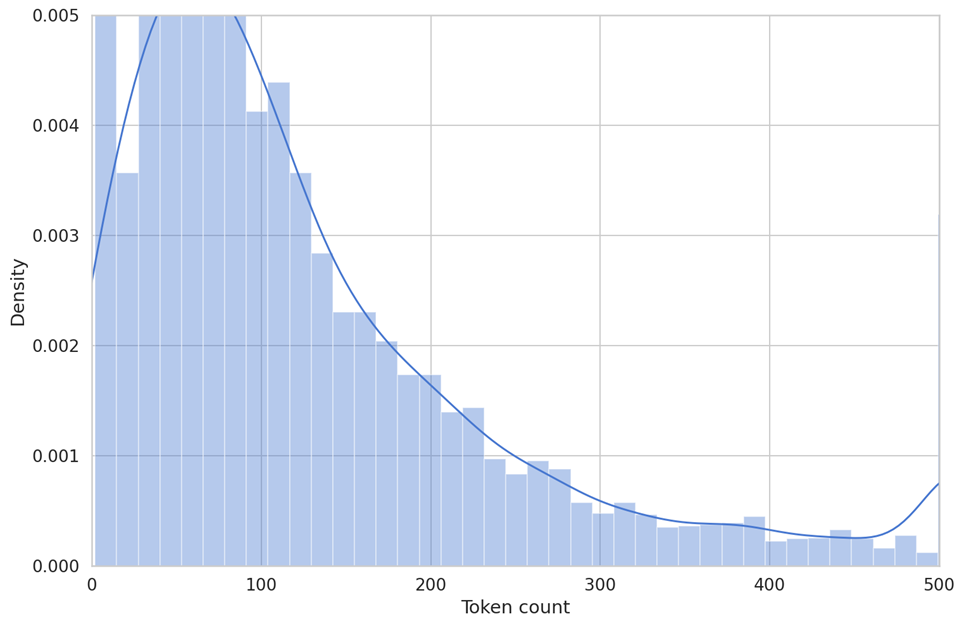
\includegraphics[width=1\textwidth]{images/512.png}
\caption{\gls{Ktrain} learner plot}
\label{fig:fig_07}
\end{figure}
\FloatBarrier

From Figure~\ref{fig:fig_07} it is possible to see that after 400 tokens the density is less than 0.001. For this reason I can set max len to 400.

\subsubsection{Build a model and wrap in learner}
\label{chap:ktrain build a model}
The section describes the construction of the model using the \gls{Ktrain} library.

\paragraph{Model}
My choice fell on dbmz/bert-german-cased.
This is one of the best models I found on \gls{Hugging Face} \cite{noauthor_dbmdzbert-base-german-uncased_nodate}, from the site it is possible to read that:
\begin{quote}
    The source data for the model consists of a recent Wikipedia dump, EU Bookshop corpus, Open Subtitles, CommonCrawl, ParaCrawl and News Crawl. This results in a dataset with a size of 16GB and 2,350,234,427 tokens.
\end{quote}

As the git name suggests dbmz \cite{noauthor_open_nodate} is available as open-source from the MDZ Digital Library team at the Bavarian State Library \cite{noauthor_munich_nodate} based in Munich. Dbmz is one of the leading exponents of the German language and more.

In order to work with \gls{Ktrain}, I then had to set the model's name:

 \begin{tcolorbox}[breakable, size=fbox, boxrule=1pt, pad at break*=1mm,colback=cellbackground, colframe=cellborder]
\begin{Verbatim}[commandchars=\\\{\},fontsize=\footnotesize]
\PY{n}{MODEL\PYZus{}NAME} \PY{o}{=} \PY{l+s+s1}{\PYZsq{}}\PY{l+s+s1}{dbmdz/bert\PYZhy{}base\PYZhy{}german\PYZhy{}cased}\PY{l+s+s1}{\PYZsq{}}
\end{Verbatim}
\end{tcolorbox}

From the \gls{Ktrain} documentation it is possible to understand how to use the library.
The text.Transformer() function allows me to do text classification using a \gls{Hugging Face} transformers.

    \begin{tcolorbox}[breakable, size=fbox, boxrule=1pt, pad at break*=1mm,colback=cellbackground, colframe=cellborder]
\begin{Verbatim}[commandchars=\\\{\},fontsize=\footnotesize]
\PY{n}{t} \PY{o}{=} \PY{n}{text}\PY{o}{.}\PY{n}{Transformer}\PY{p}{(}\PY{n}{MODEL\PYZus{}NAME}\PY{p}{,} \PY{n}{maxlen}\PY{o}{=}\PY{l+m+mi}{400}\PY{p}{,} \PY{n}{class\PYZus{}names}\PY{o}{=}\PY{p}{[}\PY{l+s+s1}{\PYZsq{}}\PY{l+s+s1}{0}\PY{l+s+s1}{\PYZsq{}}\PY{p}{,}\PY{l+s+s1}{\PYZsq{}}\PY{l+s+s1}{1}\PY{l+s+s1}{\PYZsq{}}\PY{p}{]}\PY{p}{)}
\end{Verbatim}
\end{tcolorbox}

The t.preprocess() function allows me to use the transformer to tokenize and encode the train and test datasets.
    \begin{tcolorbox}[breakable, size=fbox, boxrule=1pt, pad at break*=1mm,colback=cellbackground, colframe=cellborder]
\begin{Verbatim}[commandchars=\\\{\},fontsize=\footnotesize]
\PY{n}{trn} \PY{o}{=} \PY{n}{t}\PY{o}{.}\PY{n}{preprocess\PYZus{}train}\PY{p}{(}\PY{n}{xtrain\PYZus{}list}\PY{p}{,}\PY{n}{ytrain\PYZus{}list}\PY{p}{)}
\end{Verbatim}
\end{tcolorbox}

    \begin{Verbatim}[commandchars=\\\{\},fontsize=\footnotesize]
preprocessing train{\ldots}
language: de
train sequence lengths:
        mean : 105
        95percentile : 317
        99percentile : 623
    \end{Verbatim}

    \begin{Verbatim}[commandchars=\\\{\},fontsize=\footnotesize]
Is Multi-Label? False
    \end{Verbatim}

    \begin{tcolorbox}[breakable, size=fbox, boxrule=1pt, pad at break*=1mm,colback=cellbackground, colframe=cellborder]
\begin{Verbatim}[commandchars=\\\{\},fontsize=\footnotesize]
\PY{n}{val} \PY{o}{=} \PY{n}{t}\PY{o}{.}\PY{n}{preprocess\PYZus{}test}\PY{p}{(}\PY{n}{xtest\PYZus{}list}\PY{p}{,} \PY{n}{ytest\PYZus{}list}\PY{p}{)}
\end{Verbatim}
\end{tcolorbox}

    \begin{Verbatim}[commandchars=\\\{\},fontsize=\footnotesize]
preprocessing test{\ldots}
language: de
test sequence lengths:
        mean : 111
        95percentile : 342
        99percentile : 619
    \end{Verbatim}
    
My model is nothing more than a wrap of all the previous steps, added to the get\_classifier() function:  
    \begin{tcolorbox}[breakable, size=fbox, boxrule=1pt, pad at break*=1mm,colback=cellbackground, colframe=cellborder]
\begin{Verbatim}[commandchars=\\\{\},fontsize=\footnotesize]
\PY{n}{model} \PY{o}{=} \PY{n}{t}\PY{o}{.}\PY{n}{get\PYZus{}classifier}\PY{p}{(}\PY{p}{)}
\end{Verbatim}
\end{tcolorbox}


\paragraph{get\_learner}
Now that I have a model, I can create a learner. A learner object will be used to help tune and train my network.
    \begin{tcolorbox}[breakable, size=fbox, boxrule=1pt, pad at break*=1mm,colback=cellbackground, colframe=cellborder]
\begin{Verbatim}[commandchars=\\\{\},fontsize=\footnotesize]
\PY{n}{learner} \PY{o}{=} \PY{n}{ktrain}\PY{o}{.}\PY{n}{get\PYZus{}learner}\PY{p}{(}\PY{n}{model}\PY{p}{,} \PY{n}{train\PYZus{}data}\PY{o}{=}\PY{n}{trn}\PY{p}{,} \PY{n}{val\PYZus{}data}\PY{o}{=}\PY{n}{val}\PY{p}{,} \PY{n}{batch\PYZus{}size}\PY{o}{=}\PY{l+m+mi}{12}\PY{p}{)}
\end{Verbatim}
\end{tcolorbox}
\subsubsection{Model training}
\label{chap:model training}
\paragraph{learner.lr\_find and plot()}
With a learner object, I can simulate a workout on different learning rates, so I can see the best one, I will use the function:
    \begin{tcolorbox}[breakable, size=fbox, boxrule=1pt, pad at break*=1mm,colback=cellbackground, colframe=cellborder]
\begin{Verbatim}[commandchars=\\\{\},fontsize=\footnotesize]
\PY{n}{learner}\PY{o}{.}\PY{n}{lr\PYZus{}find}\PY{p}{(}\PY{p}{)}
\end{Verbatim}
\end{tcolorbox}


With the learner.lr\_plot() function I can \gls{plot} the graph of what I just trained, so can I visually inspect the loss \gls{plot} to help identify the maximal learning rate associated with falling loss.
Figure~\ref{fig:fig_08} shows how it works:
 \begin{tcolorbox}[breakable, size=fbox, boxrule=1pt, pad at break*=1mm,colback=cellbackground, colframe=cellborder]
\begin{Verbatim}[commandchars=\\\{\},fontsize=\footnotesize]
\PY{n}{learner}\PY{o}{.}\PY{n}{lr\PYZus{}plot}\PY{p}{(}\PY{p}{)}
\end{Verbatim}
\end{tcolorbox}

\begin{figure}[ht!]
\centering
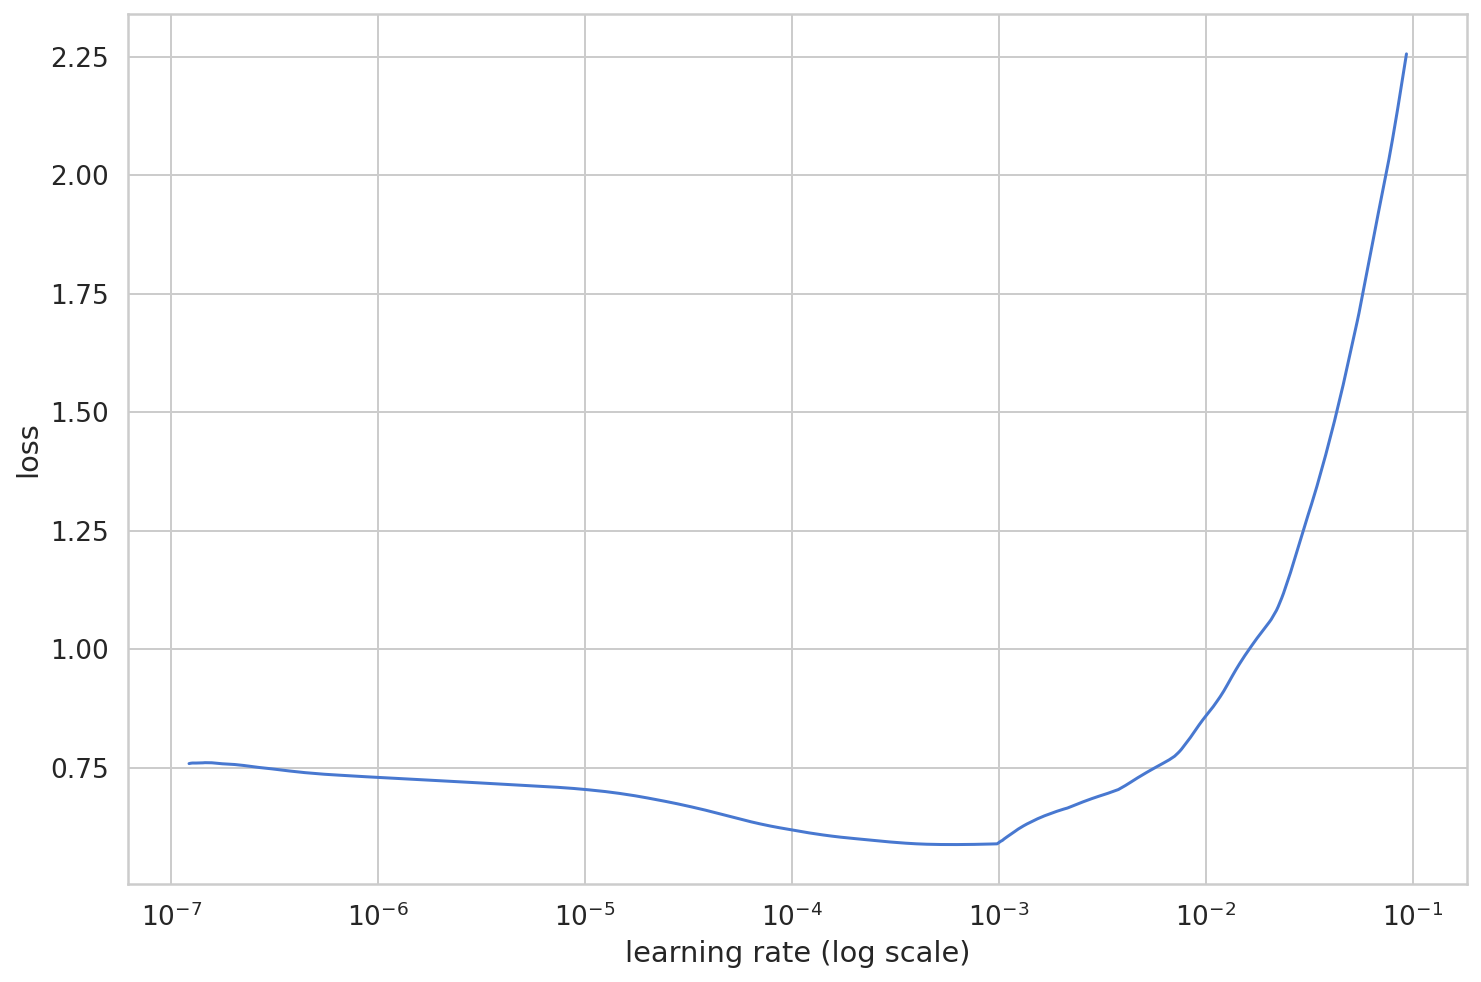
\includegraphics[width=1\textwidth]{images/output_118_1.png}
\caption{\gls{Ktrain} learner plot}
\label{fig:fig_08}
\end{figure}
\FloatBarrier

\paragraph{Autofit}
Now I am going to use the autofit \cite{noauthor_amaiyaktrainautofit_nodate} method to train the model with the parameters I found earlier.
The autofit method uses a cyclical learning rate schedule. The default learning rate is the triangular learning rate policy \cite{smith_cyclical_2017}.
As before, I invoked the help function to better understand how the autofit function works.
The autofit method accepts two primary arguments, learning rate and epochs.
If epochs are not defined then the method will train until the validation loss no longer improves after a certain period. This period is also configurable using the early\_stopping argument. 

I also used another two arguments, reduce\_on\_plateau and checkpoint\_folder.\\
reduce\_on\_plateau check if the validation loss fails to improve after a specified number of epochs.
checkpoint\_folder folder path in which to save the model weights for each epoch.\\
Next, I called the function as below:
    \begin{tcolorbox}[breakable, size=fbox, boxrule=1pt, pad at break*=1mm,colback=cellbackground, colframe=cellborder]
\begin{Verbatim}[commandchars=\\\{\},fontsize=\footnotesize]
\PY{n}{learner}\PY{o}{.}\PY{n}{autofit}\PY{p}{(}\PY{l+m+mf}{3e\PYZhy{}5}\PY{p}{,} \PY{n}{reduce\PYZus{}on\PYZus{}plateau}\PY{o}{=}\PY{l+m+mi}{3}\PY{p}{,} \PY{n}{checkpoint\PYZus{}folder}\PY{o}{=}\PY{l+s+s1}{\PYZsq{}}\PY{l+s+s1}{./checkpointNewModel25.04/}\PY{l+s+s1}{\PYZsq{}}\PY{p}{)}
\end{Verbatim}
\end{tcolorbox}


  \begin{Verbatim}[commandchars=\\\{\},fontsize=\footnotesize]
early\_stopping automatically enabled at patience=5


begin training using triangular learning rate policy with max lr of 3e-05{\ldots}
Epoch 1/1024
472/472 [==============================] - 190s 378ms/step - loss: 0.4936 -
accuracy: 0.7200 - val\_loss: 0.1846 - val\_accuracy: 0.9300
Epoch 2/1024
472/472 [==============================] - 178s 375ms/step - loss: 0.1627 -
accuracy: 0.9432 - val\_loss: 0.1748 - val\_accuracy: 0.9350
...
...
Epoch 00005: Reducing Max LR on Plateau: new max lr will be 1.5e-05 (if not
early\_stopping).
Epoch 6/1024
472/472 [==============================] - 178s 376ms/step - loss: 0.0299 -
accuracy: 0.9921 - val\_loss: 0.2663 - val\_accuracy: 0.9307
Epoch 7/1024
472/472 [==============================] - 179s 376ms/step - loss: 0.0178 -
accuracy: 0.9949 - val\_loss: 0.2605 - val\_accuracy: 0.9314
Restoring model weights from the end of the best epoch.
Epoch 00007: early stopping
Weights from best epoch have been loaded into model.
    \end{Verbatim}
    
\subsubsection{Results}
\paragraph{Validate}
Using the:
    \begin{tcolorbox}[breakable, size=fbox, boxrule=1pt, pad at break*=1mm,colback=cellbackground, colframe=cellborder]
\begin{Verbatim}[commandchars=\\\{\},fontsize=\footnotesize]
\PY{n}{learner}\PY{o}{.}\PY{n}{validate}\PY{p}{(}\PY{p}{)}
\end{Verbatim}
\end{tcolorbox}method I can create a \gls{Confusion matrix} on the newly trained data in order to get a more detailed picture:
    \begin{Verbatim}[commandchars=\\\{\},fontsize=\footnotesize]
              precision    recall  f1-score   support

           0       0.94      0.93      0.94       725
           1       0.93      0.94      0.93       690

    accuracy                           0.93      1415
   macro avg       0.93      0.94      0.93      1415
weighted avg       0.94      0.93      0.93      1415

    \end{Verbatim}
            \begin{tcolorbox}[breakable, size=fbox, boxrule=.5pt, pad at break*=1mm, opacityfill=0]
\begin{Verbatim}[commandchars=\\\{\},fontsize=\footnotesize]
array([[14883,  2497],
       [ 2610, 14915]])
\end{Verbatim}
\end{tcolorbox}


\textbf{What is a \gls{Confusion matrix}?}

\gls{Confusion matrix} is one of the easiest and most intuitive metrics to check the \gls{accuracy} of a model.
It is mostly used for classification problems, as in my example.

The \gls{Confusion matrix} is calculated as shown in Figure~\ref{fig:fig_cm}:
\begin{figure}[ht!]
\centering
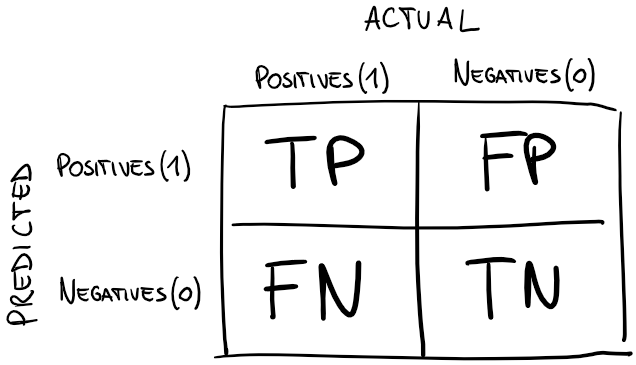
\includegraphics[width=0.5\textwidth]{images/cm.png}
\caption{\gls{Confusion matrix}}
\label{fig:fig_cm}
\end{figure}
\FloatBarrier
In my case I have the two classes 0 (negative) and 1 (positive).

\textbf{True Positive(TP)}: number of cases in which the value of the real data is 1 (positive) and the prediction of the model is also 1. Correct prediction.

\textbf{True Negative(TN)}: number of the real cases is 0 (negative) and the cases predicted from the model are 0. Correct prediction.

\textbf{False Positive(FP)}: number of the real cases are 0 (negative) and the cases predicted from the model are 1 (positive). Wrong prediction. 

\textbf{False Negative(FN)}: number of the real cases are 1 (positive) and the cases predicted from the model are 0 (negative). Wrong prediction. 

Thanks to the \gls{Confusion matrix}, several factors can be calculated:
\begin{itemize}
    \item \gls{accuracy}
    \item precision
    \item \gls{recall} or sensitivity
    \item \gls{F1 score}.
\end{itemize}

\textbf{Accuracy} \cite{brownlee_how_2020}:\\
This metric, when talking about tasks such as classification, is the number of correct predictions made by the model, out of all the predictions made.
Figure~\ref{fig:fig_acc} shows how this metric is calculated:
\begin{figure}[ht!]
\centering
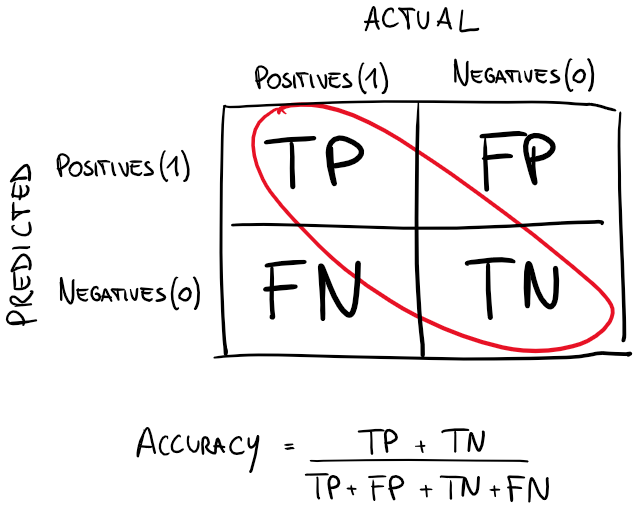
\includegraphics[width=0.5\textwidth]{images/acc.png}
\caption{Accuracy}
\label{fig:fig_acc}
\end{figure}
\FloatBarrier

Accuracy is a good measure when the classes of targets in the data are nearly balanced. 
For example class A= 60\% and class B= 40\%. 
If instead I have a big difference like, class A = 85\% and class B=15\% the \gls{accuracy} cannot be used because it is not a reliable value.

For this reason I made a resample of my dataset, to have small difference between the two classes. See \ref{chap:resample}.

In my case I have a great \gls{accuracy} (93\%) counting that the model is based on a language where punctuation, cased and uncased words have a great influence, I can be satisfied.


\textbf{Precision} \cite{brownlee_how_2020}:\\
Precision is the ratio of correctly predicted positive observations to the total predicted positive observations. 
The question that this metric answers is: 
of all the articles labelled as positive, how many of them are actually positive?

High \gls{precision} relates to the low false positive (FP) rate. 
Figure~\ref{fig:fig_pre} shows how this metric is calculated:
\begin{figure}[ht!]
\centering
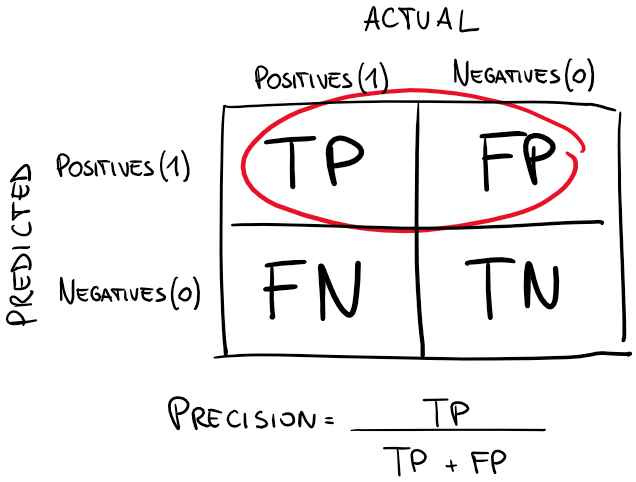
\includegraphics[width=0.5\textwidth]{images/prec.png}
\caption{\gls{precision}}
\label{fig:fig_pre}
\end{figure}
\FloatBarrier

Precision is used in cases where we need to be certain, so it is not the quantity that matters but the quality. For example, if I must make a prediction about cancer cases, I must be 100\% sure that it is correct even if it is only one case.
In my case it is better to have great \gls{accuracy}, but if I have mistaken, I do not have repercussions like for example in the medical field.

In my case \gls{precision} (0 = 94\%, 1 = 93\%) is aligned with all other values.

\textbf{Recall (or Sensitivity)} \cite{brownlee_how_2020}:\\
Recall is the ratio of correctly predicted positive observations to all observations in actual class. It answers the question:
of all the articles that are truly positive, how many of them were predicted correctly? 
Figure~\ref{fig:fig_rec} shows how this metric is calculated:
\begin{figure}[ht!]
\centering
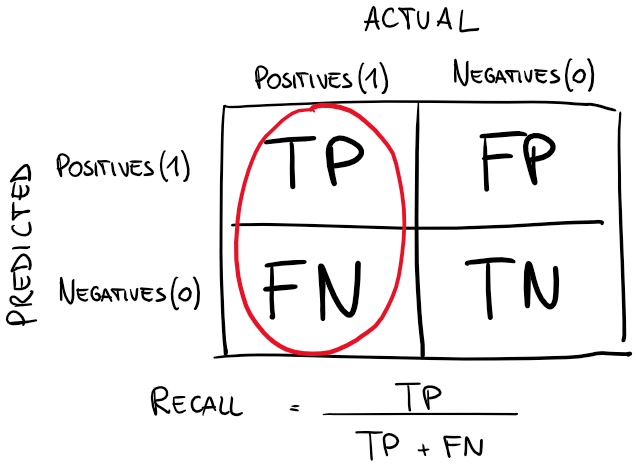
\includegraphics[width=0.5\textwidth]{images/rec.png}
\caption{Recall/Sensitivity}
\label{fig:fig_rec}
\end{figure}
\FloatBarrier

Recall is used not so much to figure out which cases were predicted correctly, but more the capture of all "positive sentiment" cases with the answer as "positive".

In my case \gls{recall} (0 = 93\%, 1 = 94\%) is aligned with all other values.

\textbf{F1 score} \cite{brownlee_how_2020}:\\
We need a metric that takes \gls{precision} and \gls{recall} into account, that's why \gls{F1 score} exists.
\gls{F1 score} is the weighted average of \gls{precision} and \gls{recall}.
Figure~\ref{fig:fig_f1} shows how this metric is calculated:
\begin{figure}[ht!]
\centering

\includegraphics[width=0.4\textwidth]{images/f1.png}
\caption{\gls{F1 score}}
\label{fig:fig_f1}
\end{figure}
\FloatBarrier

\gls{F1 score} is usually more useful than \gls{accuracy}, especially if we have an uneven class distribution. Accuracy works best if false positives and false negatives have similar cost. If the cost of false positives and false negatives are very different, it is better to look at both \gls{precision} and \gls{recall}.

In my case \gls{F1 score} (0 = 94\%, 1 = 93\%) is aligned with all other values.


\subsubsection{Save and reload model}
Thanks to the last update of \gls{Ktrain} in March, to save the trained model and its weights I will simply use:
    \begin{tcolorbox}[breakable, size=fbox, boxrule=1pt, pad at break*=1mm,colback=cellbackground, colframe=cellborder]
\begin{Verbatim}[commandchars=\\\{\},fontsize=\footnotesize]
\PY{n}{predictor}\PY{o}{.}\PY{n}{save}\PY{p}{(}\PY{l+s+s1}{\PYZsq{}}\PY{l+s+s1}{./modelsave/bertDe\PYZus{}predictor\PYZus{}93}\PY{l+s+s1}{\PYZsq{}}\PY{p}{)}
\end{Verbatim}
\end{tcolorbox}

Even simpler is to load a model, in fact used the function load\_predictor() by specifying from which path to take the model, I can already in the next line make predictions.
\begin{tcolorbox}[breakable, size=fbox, boxrule=1pt, pad at break*=1mm,colback=cellbackground, colframe=cellborder]
\begin{Verbatim}[commandchars=\\\{\},fontsize=\footnotesize]
\PY{c+c1}{\PYZsh{} reload predictor}
\PY{n}{predictor} \PY{o}{=} \PY{n}{ktrain}\PY{o}{.}\PY{n}{load\PYZus{}predictor}\PY{p}{(}\PY{l+s+s1}{\PYZsq{}}\PY{l+s+s1}{./modelsave/bertDe\PYZus{}predictor\PYZus{}93}\PY{l+s+s1}{\PYZsq{}}\PY{p}{)}
\PY{n}{predictor}\PY{o}{.}\PY{n}{predict}\PY{p}{(}\PY{l+s+s1}{\PYZsq{}}\PY{l+s+s1}{Heute ist ein schöner Tag.}\PY{l+s+s1}{\PYZsq{}}\PY{p}{)}
\end{Verbatim}
\end{tcolorbox}


\subsection{Newspaper API's}
\label{chap:news apis}
Now that I have a trained and working model, what I am missing is data from Swiss newspapers.
To do this I used some Application Programming Interfaces (API):
\begin{itemize}
    \item NewsAPI \cite{noauthor_news_nodate}
    \item GNewsAPI \cite{noauthor_gnews_nodate}
\end{itemize}

I have used both APIs in developer mode for free.

NewsAPI allows me to:
\begin{itemize}
    \item search all articles and get live top headlines,
    \item new articles available with 1 hour delay,
    \item search articles up to a month old,
    \item 100 requests per day,
    \item No extra requests available,
    \item No uptime SLA,
    \item Basic support.
\end{itemize}

GnewAPI allows me to:
\begin{itemize}
    \item 100 requests per day,
    \item basic support,
    \item up to 10 articles returned per request,
    \item maximum of 1 request per second.
\end{itemize}
The main idea was to use the API in a Python file, so that I have the news of the day every time I launch the file.
I used two APIs because I have limitations on the number of requests per day and the number of items per request.
To avoid these limitations I imported both APIs in a single Python file, for each API I made a request per category and saved the response in json.
Categories are:
\begin{itemize}
    \item world,
    \item nation,
    \item business,
    \item technology,
    \item entertainment,
    \item sports,
    \item science,
    \item health.
\end{itemize}

I transformed the jsons into dataframes, for each dataframe I checked to make sure they were not empty and deleted the columns I did not need.
I noticed that NewsAPI returns only newspapers in German language even if I change the settings.

Once I have the different clean dataframes I put them in a list and merge them into one dataframe thanks to the \gls{Pandas} concat() function.
I then check the list that there are no duplicates, and if there are I delete them, always thanks to \gls{Pandas} with the drop\_duplicates() function.

By doing so I expect to have about 30 articles in German for each category.

At this point still using \gls{Pandas} to\_csv, I export and save the dataframe in csv format with its timestamp.

In order to have more freedom I export not only the concatenated dataframe, but also each individual dataframe category.

Now that I have a working Python script what I need is just to make it automatic in order to make one request per day.
Using the virtual machine always active, I created, thanks to the windows task scheduler, a task that would start my script once a day and save the files in a certain folder.

\subsection{Model test with newspaper data}
\label{chap:model test newspaper}
\subsubsection{Ground truth}
After a few days of scraping data thanks to my script, I decided to do some tests with the model I had trained. 
First, I imported the data into my environment, then thanks to \gls{Pandas} I started to analyze it and then I made the predictions.
The dataset I imported has the following columns:
\begin{itemize}
    \item source
    \item title
    \item description
\end{itemize}

Before I can look at the model results, I need to create a ground truth.
In the data science world, it is called "ground truth" when I compare a result created by a user "by hand" with what the model predicted.
This is to be able to compare the real data with the data from the model. 
So, I took a sample of a dataset, and hand classified a positive or negative sentiment for each newspaper article.
I started by ranking the sentiment at the description of each article without reading the title first, and then did the same at the title, independent of the description. I did this because some descriptions without reading the title were of one sentiment, but with title attached were of the opposite sentiment.
One problem with sentiment prediction I had when the article was "a fact". Normally it can be interpreted as neutral. In that case it can be both, I kept right whether the model predicted positive or negative.

Once I have a ground truth, I tested the model and had it make predictions on the description column, and then on the title column.

These were the results:

\begin{longtable}[c]{|l|l|l|l|}
\hline
\textbf{Model} & \textbf{Accuracy} & \textbf{Target} & \textbf{Score} \\ \hline
\endfirsthead
%
\multicolumn{4}{c}%
{{\bfseries Table \thetable\ continued from previous page}} \\
\hline
\textbf{Model} & \textbf{Accuracy} & \textbf{Target} & \textbf{Score} \\ \hline
\endhead
%
\gls{Ktrain}   Automatic & 90\% & description & 22/30 \\ \hline
\gls{Ktrain}   Manual & 93\% & description & 26/30 \\ \hline
\gls{Ktrain} Manual & 93\% & title & 29/30 \\ \hline
\caption{Model comparison}
\label{tab:table-model}\\
\end{longtable}

\subsubsection{Interesting case studies}
In Figure~\ref{fig:fig_09} it is possible to see the comparison between the models: 
\begin{figure}[H]
\centering
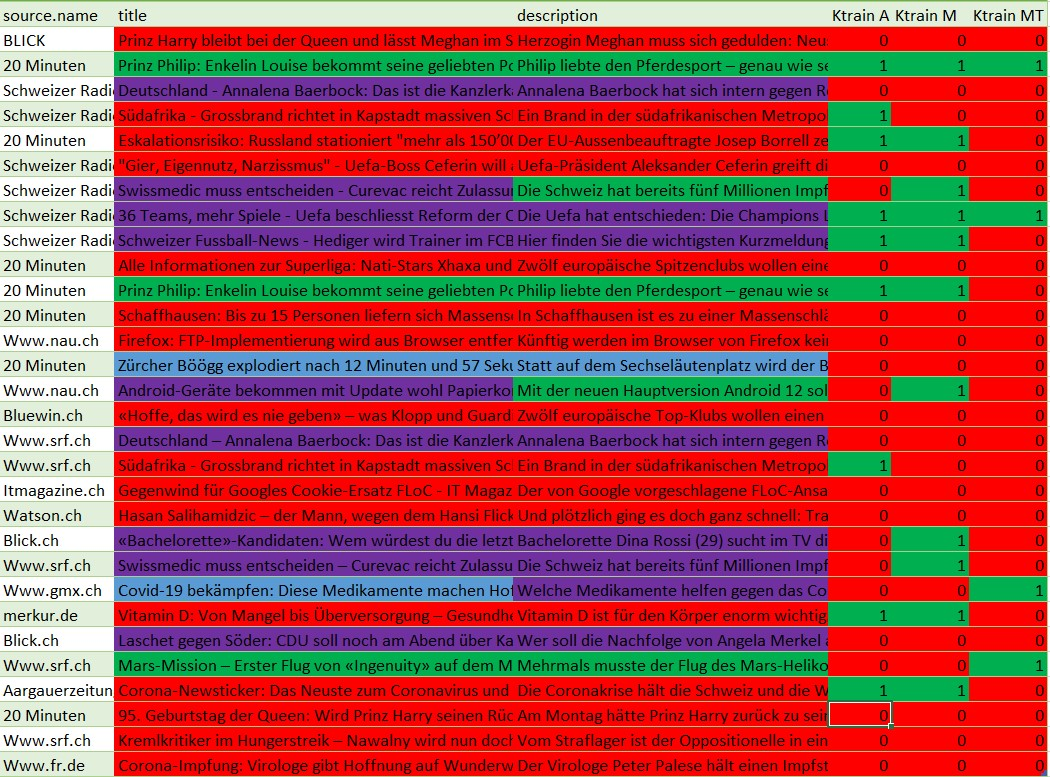
\includegraphics[width=1\textwidth]{images/ktrainmanual.jpg}
\caption{Model Comparison}
\label{fig:fig_09}
\end{figure}
\FloatBarrier
The colors in the columns title and description refer to the manual labelling.
The red and green colors refer to negative(0) or positive(1), purple instead are the neutral cases where a sentiment cannot be defined, so both values from the model I considered them correct.
In blue are in interesting cases, because the text without a context comes across as negative, in fact it is not.

\paragraph{Example:}
"Statt auf dem Sechseläutenplatz wird der Böögg dieses Jahr im Kanton Uri verbrannt. Der Wind sorgte dafür, dass der Kopf schnell explodierte. Der Sommer kann kommen!"

The model classifies this sentence negative for obvious reasons:
something is burned, head exploded, I personally had to inform myself because even I without context was not sure how to classify this news. This shows that the machine is not perfect and cannot understand shades that are difficult even to humans.

\subsubsection{Find the bug}
What can be seen is that the description alone is often predicted positively compared to the title which is predicted negatively.
For this reason the next test sees the \gls{Ktrain} Manual model doing prediction on "title+description" together, to see if the results improve.

The \gls{accuracy} of this prediction improved considerably, although I often encountered trivial errors.
So what I did was to use predictor.explain() so I could better understand how the model works and I did several tests.

With predictor.explain() I can generate a visualization.
The visualization technique is called "Explain like I’m 5" (ELI5)\cite{noauthor_textexplainer_nodate} and uses the Local Interpretable Model-agnostic Explanations (LIME) algorithm \cite{ribeiro_why_2016}\cite{ribeiro_marcotcrlime_2021}, in which the importance of each single word can be seen based on the final prediction, using an interpretable linear model.
The green words are inferred as contributing to the classification. The red (or pink) words detract from our final prediction. (Shade of color denotes the strength or size of the coefficients in the inferred linear model.)

I created a dataset on purpose with the newspaper header with more data, to be able to make a good comparison.
So, I chose "20 Minuten" to be able to do some tests.

This dataframe has on both "title+description" and "description" 26 negative predictions and 13 positive predictions, while on "title" it has 33 negatives and 6 positives, perfect for understanding what is going on.

Since on both "title+description" and "description" the results match, I focus on the "title" column.

Looking in the dataframe it can be seen that NewsAPI adds at the end of the headline "- newspaper name".

Before making the tests, there are to explain some data that help to understand better how the model works.
\begin{itemize}
    \item \textbf{y=} refers to how the text has been classified, it can be 0 (negative) or 1 (positive),
    \item \textbf{score} is the score that the sentence has obtained looking at the Feature contribution. If the score is negative then y=0 if positive y=1. Higher is the score, higher is the probability value.
    \item \textbf{Contribution} = (weight * feature value) is calculated for each value. For feature values we can have 2 types of features:
    \begin{itemize}
        \item \textbf{Highlighted in text(sum)},
        \item \textbf{<BIAS>}
    \end{itemize}
    Both of these values can be positive or negative, green or red.
    "Highlighted in text(sum)" indicates the correct feature, while "BIAS" incorrect. These two values are summed together, they can have the same or opposite sign.
\end{itemize}

I did 4 tests on the same sentence with positive ground truth:
\begin{enumerate}
  \item Title with source at the end = \textbf{negative 0.632}
  \begin{figure}[H]
\centering
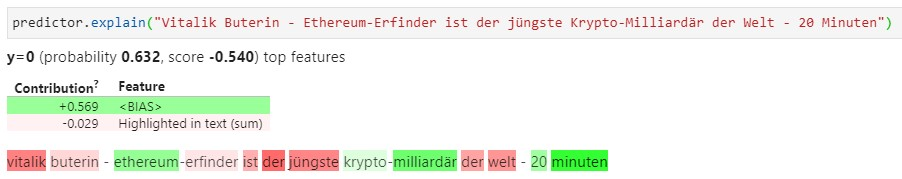
\includegraphics[width=1\textwidth]{images/1text.jpg}
\caption{predictor.explain() test 1}
\label{fig:fig_001}
\end{figure}
\FloatBarrier
The model classifies it as negative, why?
BIAS = +0.569, (incorrect)\\
Highlighted in text(sum) = -0.029, (correct)\\
Score will then be = 0.029 - 0.569 = -0.540.\\
Having negative score, y = 0 with probability = 0.632.

  \item Title without source at the end = \textbf{positive 0.583}
    \begin{figure}[H]
\centering
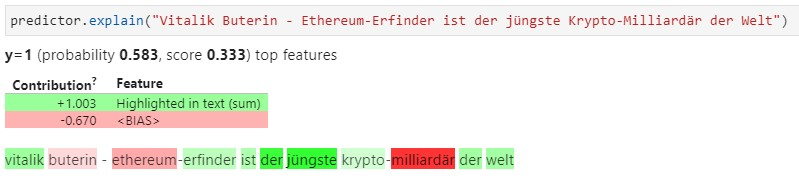
\includegraphics[width=1\textwidth]{images/3text.jpg}
\caption{predictor.explain() test 2}
\label{fig:fig_002}
\end{figure}
\FloatBarrier
Highlighted in text(sum) = +1.003, (correct)\\
BIAS = -0.670, (incorrect)\\
Score will then be = 1.003 - 0.670 = 0.333.\\
Having positive score, y = 1 with probability = 0.583.

\textit{I tried adding punctuation:}
  \item Title with source at the end and no dot = \textbf{positive 0.617}
      \begin{figure}[H]
\centering
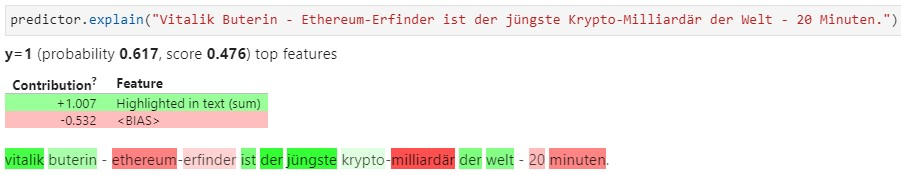
\includegraphics[width=1\textwidth]{images/2text.jpg}
\caption{predictor.explain() test 3}
\label{fig:fig_003}
\end{figure}
\FloatBarrier
Highlighted in text(sum) = +1.007, (correct)\\
BIAS = -0.532, (incorrect)\\
Score will then be = 1.007 - 0.532 = 0.476.\\
Having positive score, y = 1 with probability = 0.617.
  \item Title without source at the end with dot = \textbf{positive 0.849}
      \begin{figure}[H]
\centering
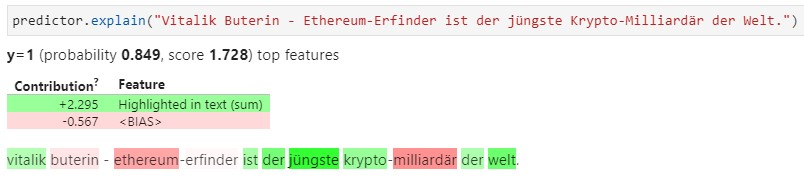
\includegraphics[width=1\textwidth]{images/4text.jpg}
\caption{predictor.explain() test 4}
\label{fig:fig_004}
\end{figure}
\FloatBarrier
Highlighted in text(sum) = +2.295, (correct)\\
BIAS = -0.567, (incorrect)\\
Score will then be = 2.295 - 0.567 = 1.728.\\
Having positive score, y = 1 with probability = 0.849.
\end{enumerate}

It can be understood that punctuation is very important to be able to make predictions correctly, the source already changes the meaning, but the punctuation is at the base.

I then wanted to try "title+description" with what I found previously so:
\begin{enumerate}
    \item "title+description" with “- source” with dot = \textbf{negative 0.641}
        \begin{figure}[H]
\centering
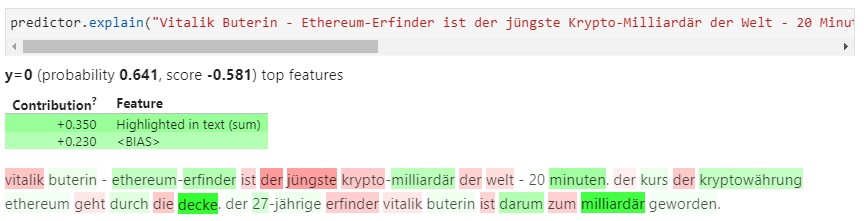
\includegraphics[width=1\textwidth]{images/5text.jpg}
\caption{predictor.explain() "title+description" with source}
\label{fig:fig_005}
\end{figure}
\FloatBarrier
In this case both BIAS and (sum) have the same sign, it means that "Highlighted in text(sum)" goes in the same direction as BIAS, so it is incorrect.
Highlighted in text(sum) = +0.230, (incorrect)\\
BIAS = +0.350, (incorrect)\\
Score will then be = -0.230 - 0.350 = -0.581.\\
Having negative score, y = 0 with probability = 0.641.
    \item "title+description" without “- source” with dot = \textbf{positive 0.578}
        \begin{figure}[H]
\centering
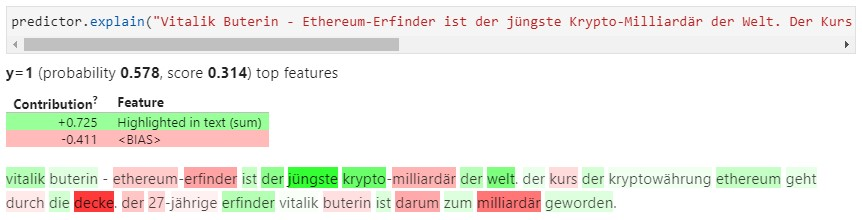
\includegraphics[width=1\textwidth]{images/6text.jpg}
\caption{predictor.explain() "title+description" without source}
\label{fig:fig_006}
\end{figure}
\FloatBarrier
Highlighted in text(sum) = +0.725, (correct)\\
BIAS = -0.411, (incorrect)\\
Score will then be = 0.725 - 0.411 = 0.314.\\
Having positive score, y = 1 with probability = 0.578.
\end{enumerate}

\textbf{Result:} Sentence with punctuation totally changes how the sentiment is predicted, while sentence without source increases the \gls{accuracy} of the predicted result.

\subsubsection{Fix the bug}
Found this "bug" there is only to understand how to proceed.
The best solution is to clean the data at the root, since NewsAPI gives me unsuitable data, I have two alternatives:
\begin{enumerate}
    \item do not use NewsAPI,
    \item try to solve the problem on data import.
\end{enumerate}

Although the first alternative is the fastest and most immediate, I opted for the second to have a good amount of data on which to make analysis.

I modified the Python script to do data scarping\footnote{\href{https://github.com/bak89/Sentiment-Analysis-on-Swiss-Newspapers/blob/main/Project\%20source/database_newspaper/gnewsapi.py}{\emph{Link GitHub "gnewsapi.py"}}}.
From the previous version I added having different categories and the timestamp of each article.
Next, I created a Python dictionary, filled with all the sources of the various newspapers, so you can clean from each title its source, if the source is not in the dictionary then a warning will notify it.
The code to do this:
\begin{tcolorbox}[breakable, size=fbox, boxrule=1pt, pad at break*=1mm,colback=cellbackground, colframe=cellborder]
\begin{Verbatim}[commandchars=\\\{\},fontsize=\footnotesize]
\PY{k}{def} \PY{n+nf}{cleanup\PYZus{}title}\PY{p}{(}\PY{n}{source}\PY{p}{,} \PY{n}{title}\PY{p}{)}\PY{p}{:}
    \PY{k}{if} \PY{n}{source} \PY{o+ow}{not} \PY{o+ow}{in} \PY{n}{SOURCES}\PY{p}{:}
        \PY{n}{logging}\PY{o}{.}\PY{n}{warn}\PY{p}{(}\PY{l+s+s2}{\PYZdq{}}\PY{l+s+s2}{Unknown source }\PY{l+s+si}{\PYZpc{}s}\PY{l+s+s2}{, leaving as\PYZhy{}is}\PY{l+s+s2}{\PYZdq{}}\PY{p}{,} \PY{n}{source}\PY{p}{)}
        \PY{n+nb}{print}\PY{p}{(}\PY{l+s+s2}{\PYZdq{}}\PY{l+s+s2}{\PYZsq{}}\PY{l+s+s2}{\PYZdq{}}\PY{o}{+}\PY{n}{source}\PY{o}{+}\PY{l+s+s2}{\PYZdq{}}\PY{l+s+s2}{\PYZsq{}}\PY{l+s+s2}{: postfix\PYZus{}title,}\PY{l+s+s2}{\PYZdq{}}\PY{p}{)}
    \PY{k}{return} \PY{n}{SOURCES}\PY{o}{.}\PY{n}{get}\PY{p}{(}\PY{n}{source}\PY{p}{,} \PY{n}{noop}\PY{p}{)}\PY{p}{(}\PY{n}{title}\PY{p}{)}
\end{Verbatim}
\end{tcolorbox}

    \begin{tcolorbox}[breakable, size=fbox, boxrule=1pt, pad at break*=1mm,colback=cellbackground, colframe=cellborder]
\begin{Verbatim}[commandchars=\\\{\},fontsize=\footnotesize]
\PY{k}{def} \PY{n+nf}{clean\PYZus{}dataframe}\PY{p}{(}\PY{n}{df}\PY{p}{)}\PY{p}{:}
    \PY{c+c1}{\PYZsh{} clean title from \PYZsq{}\PYZhy{} newspaper Name\PYZsq{}}
    \PY{n}{title\PYZus{}apply} \PY{o}{=} \PY{n}{df}\PY{o}{.}\PY{n}{apply}\PY{p}{(}
        \PY{k}{lambda} \PY{n}{row} \PY{p}{:} \PY{n}{cleanup\PYZus{}title}\PY{p}{(}\PY{n}{row}\PY{p}{[}\PY{l+s+s1}{\PYZsq{}}\PY{l+s+s1}{source.name}\PY{l+s+s1}{\PYZsq{}}\PY{p}{]}\PY{p}{,} \PY{n}{row}\PY{p}{[}\PY{l+s+s1}{\PYZsq{}}\PY{l+s+s1}{title}\PY{l+s+s1}{\PYZsq{}}\PY{p}{]}\PY{p}{)}\PY{p}{,}
        \PY{n}{axis} \PY{o}{=} \PY{l+m+mi}{1}
    \PY{p}{)}
    \PY{c+c1}{\PYZsh{} reassign column title}
    \PY{n}{df}\PY{p}{[}\PY{l+s+s1}{\PYZsq{}}\PY{l+s+s1}{title}\PY{l+s+s1}{\PYZsq{}}\PY{p}{]} \PY{o}{=} \PY{n}{title\PYZus{}apply}
    \PY{k}{return} \PY{n}{df}
\end{Verbatim}
\end{tcolorbox}

I also created a second script to concatenate all files in the same category from all days into one dataframe.
This was useful for me to be able to aggregate all the data and make the different plots. 

\subsection{Sentiment analysis on newspaper data}
\label{chap:model plot}
After managing to import, clean the data and make the prediction, I can finally do the sentiment analysis.
The sentiment analysis I will be doing will be on newspaper articles that I have previously imported and concatenated into a single dataframe, thanks to the script\footnote{\href{https://github.com/bak89/Sentiment-Analysis-on-Swiss-Newspapers/blob/main/Project\%20source/database_newspaper/Combine_CSV.py}{\emph{Link GitHub "Combine\_CSV.py"}}} I created in Python.

Now I can use my model on all the journal articles I have grouped together over time. 
I first analyzed the imported data, counting the positive and negative values that the model predicted.
By scraping from the API once a day it is very likely to have the same articles on two different days, so to have more \gls{accuracy} in the prediction I removed all duplicates.

Now I have a dataframe ready to be analyzed with the purpose of creating graphs for a better visual understanding of the data.
The first obstacle I found was to normalize the data. This means to transform the positive and negative article count, into a percentage between 0 and 100.
To do this I created two functions, the first function is related to the normalization of the entire dataframe:
\begin{tcolorbox}[breakable, size=fbox, boxrule=1pt, pad at break*=1mm,colback=cellbackground, colframe=cellborder]
\begin{Verbatim}[commandchars=\\\{\},fontsize=\footnotesize]
\PY{k}{def} \PY{n+nf}{normalize}\PY{p}{(}\PY{n}{df}\PY{p}{)}\PY{p}{:}
    \PY{c+c1}{\PYZsh{} copy the data}
    \PY{n}{df\PYZus{}max\PYZus{}scal} \PY{o}{=} \PY{n}{df}\PY{o}{.}\PY{n}{copy}\PY{p}{(}\PY{p}{)}

    \PY{c+c1}{\PYZsh{} apply normalization techniques}
    \PY{k}{for} \PY{n}{column} \PY{o+ow}{in} \PY{n}{df\PYZus{}max\PYZus{}scal}\PY{o}{.}\PY{n}{columns}\PY{p}{:}
        \PY{n}{df\PYZus{}max\PYZus{}scal}\PY{p}{[}\PY{l+s+s1}{\PYZsq{}}\PY{l+s+s1}{sentiment }\PY{l+s+s1}{\PYZpc{}}\PY{l+s+s1}{\PYZsq{}}\PY{p}{]} \PY{o}{=} \PY{p}{(}\PY{n}{df\PYZus{}max\PYZus{}scal}\PY{p}{[}\PY{l+s+s1}{\PYZsq{}}\PY{l+s+s1}{count}\PY{l+s+s1}{\PYZsq{}}\PY{p}{]} \PY{o}{/} \PY{n}{df\PYZus{}max\PYZus{}scal}\PY{p}{[}\PY{l+s+s1}{\PYZsq{}}\PY{l+s+s1}{count}\PY{l+s+s1}{\PYZsq{}}\PY{p}{]}\PY{o}{.}\PY{n}{sum}\PY{p}{(}\PY{p}{)}\PY{p}{)}\PY{o}{*}\PY{l+m+mi}{100}
        
    \PY{n}{df\PYZus{}max\PYZus{}scal}\PY{p}{[}\PY{l+s+s1}{\PYZsq{}}\PY{l+s+s1}{sentiment }\PY{l+s+s1}{\PYZpc{}}\PY{l+s+s1}{\PYZsq{}}\PY{p}{]} \PY{o}{=} \PY{n}{df\PYZus{}max\PYZus{}scal}\PY{p}{[}\PY{l+s+s1}{\PYZsq{}}\PY{l+s+s1}{sentiment }\PY{l+s+s1}{\PYZpc{}}\PY{l+s+s1}{\PYZsq{}}\PY{p}{]}\PY{o}{.}\PY{n}{round}\PY{p}{(}\PY{n}{decimals}\PY{o}{=}\PY{l+m+mi}{2}\PY{p}{)}
    \PY{k}{return} \PY{n}{df\PYZus{}max\PYZus{}scal}
    
\end{Verbatim}
\end{tcolorbox}
The second is used after a group by:


    \begin{tcolorbox}[breakable, size=fbox, boxrule=1pt, pad at break*=1mm,colback=cellbackground, colframe=cellborder]
\begin{Verbatim}[commandchars=\\\{\},fontsize=\footnotesize]
\PY{k}{def} \PY{n+nf}{norm}\PY{p}{(}\PY{n}{x}\PY{p}{)}\PY{p}{:}
    \PY{n}{x}\PY{p}{[}\PY{l+s+s1}{\PYZsq{}}\PY{l+s+s1}{sentiment }\PY{l+s+s1}{\PYZpc{}}\PY{l+s+s1}{\PYZsq{}}\PY{p}{]} \PY{o}{=} \PY{p}{(}\PY{n}{x}\PY{p}{[}\PY{l+s+s1}{\PYZsq{}}\PY{l+s+s1}{count}\PY{l+s+s1}{\PYZsq{}}\PY{p}{]} \PY{o}{/}\PY{n}{x}\PY{p}{[}\PY{l+s+s1}{\PYZsq{}}\PY{l+s+s1}{count}\PY{l+s+s1}{\PYZsq{}}\PY{p}{]}\PY{o}{.}\PY{n}{sum}\PY{p}{(}\PY{p}{)}\PY{p}{)}\PY{o}{*}\PY{l+m+mi}{100}   
    \PY{n}{x}\PY{p}{[}\PY{l+s+s1}{\PYZsq{}}\PY{l+s+s1}{sentiment }\PY{l+s+s1}{\PYZpc{}}\PY{l+s+s1}{\PYZsq{}}\PY{p}{]} \PY{o}{=} \PY{n}{x}\PY{p}{[}\PY{l+s+s1}{\PYZsq{}}\PY{l+s+s1}{sentiment }\PY{l+s+s1}{\PYZpc{}}\PY{l+s+s1}{\PYZsq{}}\PY{p}{]}\PY{o}{.}\PY{n}{round}\PY{p}{(}\PY{n}{decimals}\PY{o}{=}\PY{l+m+mi}{2}\PY{p}{)}
    \PY{k}{return} \PY{n}{x}  
\end{Verbatim}
\end{tcolorbox}

I understood the purpose of normalization through the first \gls{plot} I made. In fact, the purpose of the \gls{plot} was to see all the papers with all the positive and negative articles. The problem is that without normalization, I just rely on article count, thus losing focus on the sentiment of the newspaper.
After normalization I could then set up the plots.

Below is the list of plots I made:
\begin{itemize}
    \item \gls{plot} of sentiment positive vs negative,
    \item \gls{plot} of all newspapers positive vs negative
    \item \gls{plot} top 10 newspapers positive,
    \item \gls{plot} top 10 newspapers negative,
    \item \gls{plot} per category positive vs negative,
    \item \gls{plot} per category of the top 3 newspaper (by top 3 I mean those that have more articles),
    \item spider \gls{plot} per category of a single newspaper, 
    \item \gls{plot} in time per newspaper,
    \item \gls{plot} in time per category.
\end{itemize}

For almost all the plots I used the library \gls{Plotly}. This library is very famous in the world of data analysis and is widely used to make visualizations. 

For each \gls{plot} I created a single dataframe to leave the original dataframe intact. From the original dataframe, I then used the "group by" function of \gls{Pandas}. This function allowed me to group in a dataframe based on the values that I needed, then on the grouping calculate the normalization.

\textbf{The dataset of newspaper articles, which I used to make all the plots, have a time range from the first to the 31th of May 2021.}

\subsubsection{Plot of sentiment positive vs negative} 
The \gls{plot} in Figure~\ref{fig:fig_tot} describes the percentage of positivity and negativity of all journal articles I obtained.
\begin{figure}[H]
\centering
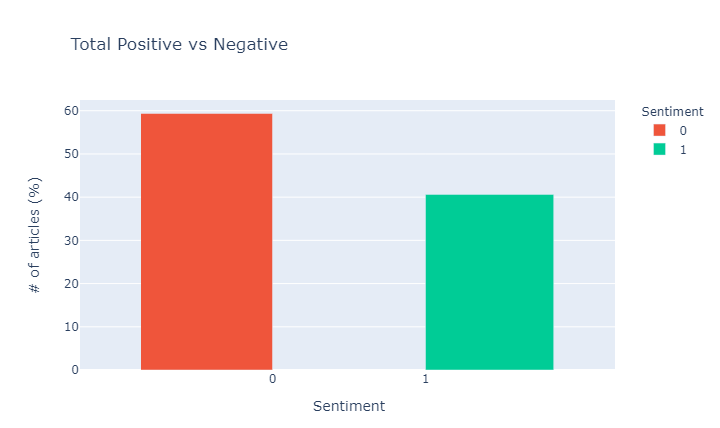
\includegraphics[width=1\textwidth]{images/tot.png}
\caption{Total positive vs negative}
\label{fig:fig_tot}
\end{figure}
\FloatBarrier

The y-axis describes the percentage of all articles with a positive or negative sentiment, which are located on the x-axis. It is visible that almost 60\% of the articles were classified with negative sentiment.

\subsubsection{Plot of all newspapers positive vs negative}
\label{chap:allposneg}
The \gls{plot} in Figure~\ref{fig:fig_all} describes the positive and negative percentage of all newspapers that have more than 5 articles, I used this filter to get more accurate statistics. Newspapers with a few articles in fact would have biased the analysis.
\begin{figure}[H]
\centering
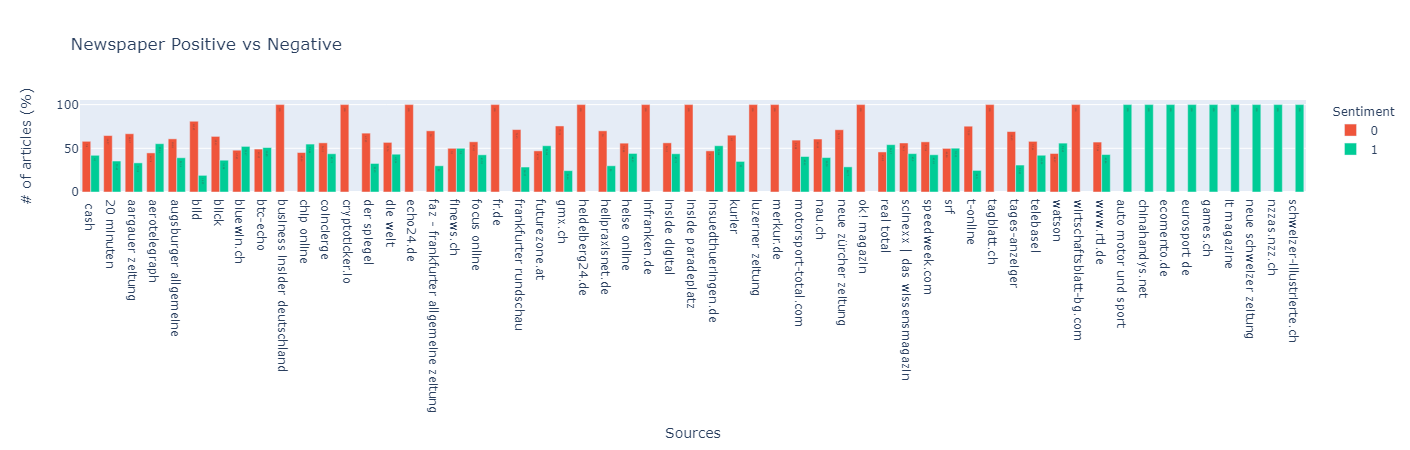
\includegraphics[width=1\textwidth]{images/posvsneg1.png}
\caption{Newspaper sentiment}
\label{fig:fig_all}
\end{figure}
\FloatBarrier
The y-axis indicates the percentage of positive or negative sentiment, categorized by the sources located on the x-axis.It is interesting to see that some newspapers have a negativity or positivity of 100\%.
For most cases, however, the negative rate is higher than the positive rate.
So not only articles but also most of the newspapers have negative sentiment.
With the next two plots it is possible to see more details.

\subsubsection{Plot top 10 newspapers positive}
The \gls{plot} in Figure~\ref{fig:fig_10pos} shows the best positive papers. The dataframe from section \ref{chap:allposneg} was used here, so newspapers below a certain number of articles are not considered.
\begin{figure}[H]
 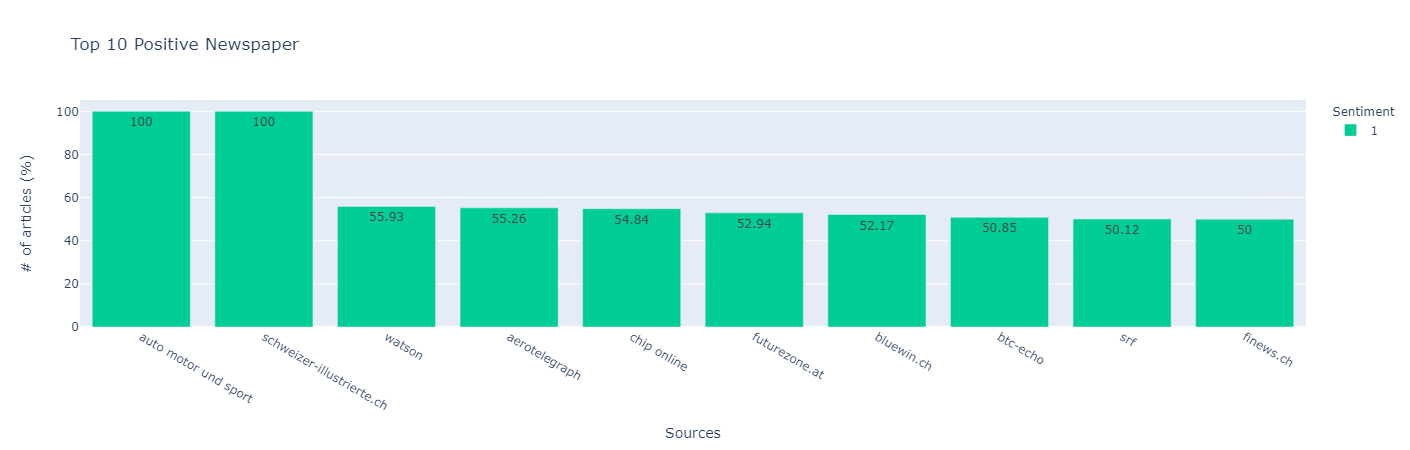
\includegraphics[width=1.25\textwidth,center]{images/toppos.png}
\caption{Top 10 positive}
\label{fig:fig_10pos}
\end{figure}
\FloatBarrier
The y-axis shows the percentage of all positive items, divided by the sources located on the x-axis.Newspapers with a car, technology or magazine theme have higher positivity.

\subsubsection{Plot top 10 newspapers negative}
The \gls{plot} in Figure~\ref{fig:fig_10neg} shows the 10 most negative newspapers. Also here the dataframe from section \ref{chap:allposneg} was used.
\begin{figure}[H]
 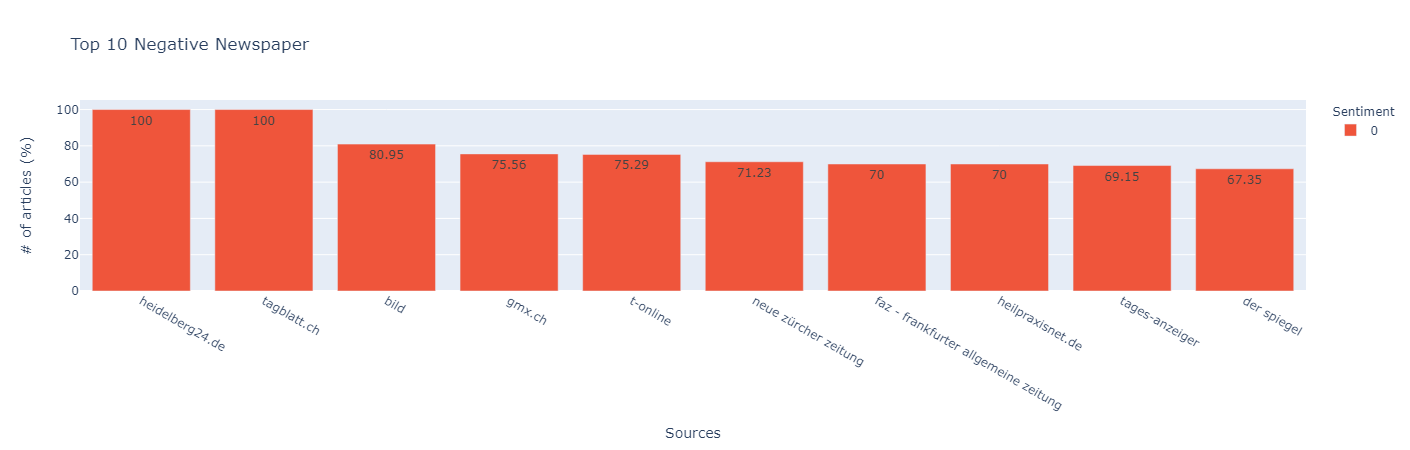
\includegraphics[width=1.25\textwidth,center]{images/topneg.png}
\caption{Top 10 negative}
\label{fig:fig_10neg}
\end{figure}
\FloatBarrier
The y-axis shows the percentage of all negative items, divided by the sources located on the x-axis.Newspapers with a regional range are the most negative.

\subsubsection{Plot per category positive vs negative}
The \gls{plot} in Figure~\ref{fig:fig_catposneg} is used to see the percentage of positivity and negativity of each category without considering the newspapers. Thanks to the grouping function I was able to group each individual category and then normalize it.

\begin{figure}[H]
 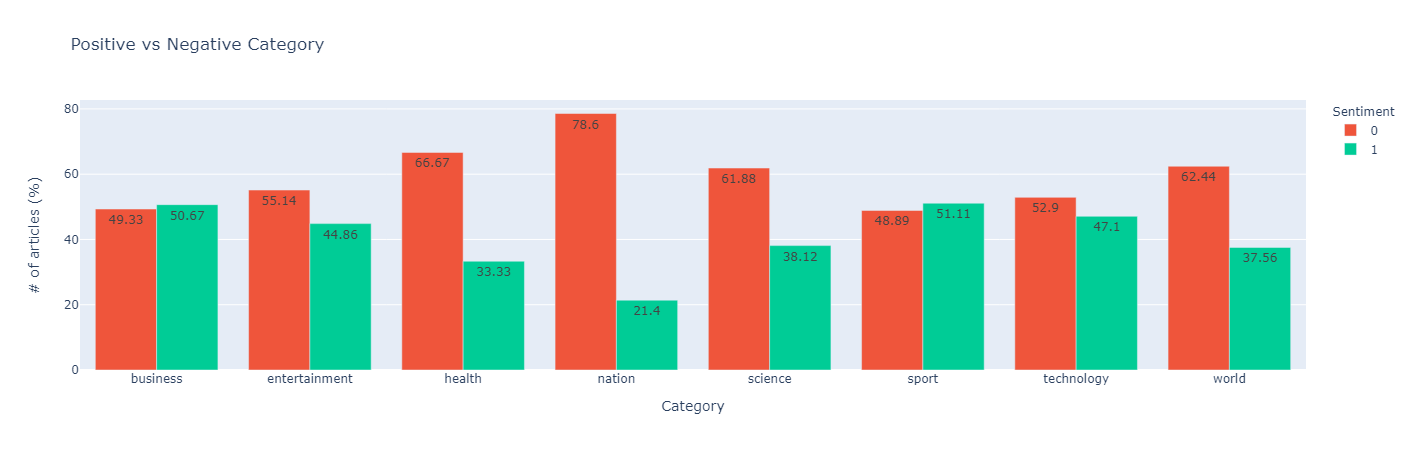
\includegraphics[width=1.25\textwidth,center]{images/cattot.png}
\caption{Category positive vs negative}
\label{fig:fig_catposneg}
\end{figure}
\FloatBarrier
The y-axis indicates the percentage of positive or negative sentiment, sorted by the categories located on the x-axis.
The category with the most negatives is "nation". Being German language newspapers, I take into account that nation means not only Switzerland, but also Germany and Austria.
Despite this, it is evident the type of negative media assault a person must endure.

\subsubsection{Plot per category of the top 3 newspapers}
The \gls{plot} in Figure~\ref{fig:fig_improvement} is used to see the percentage of positivity and negativity of the three largest newspapers by number of articles, all grouped by category.

\begin{figure}[H]
 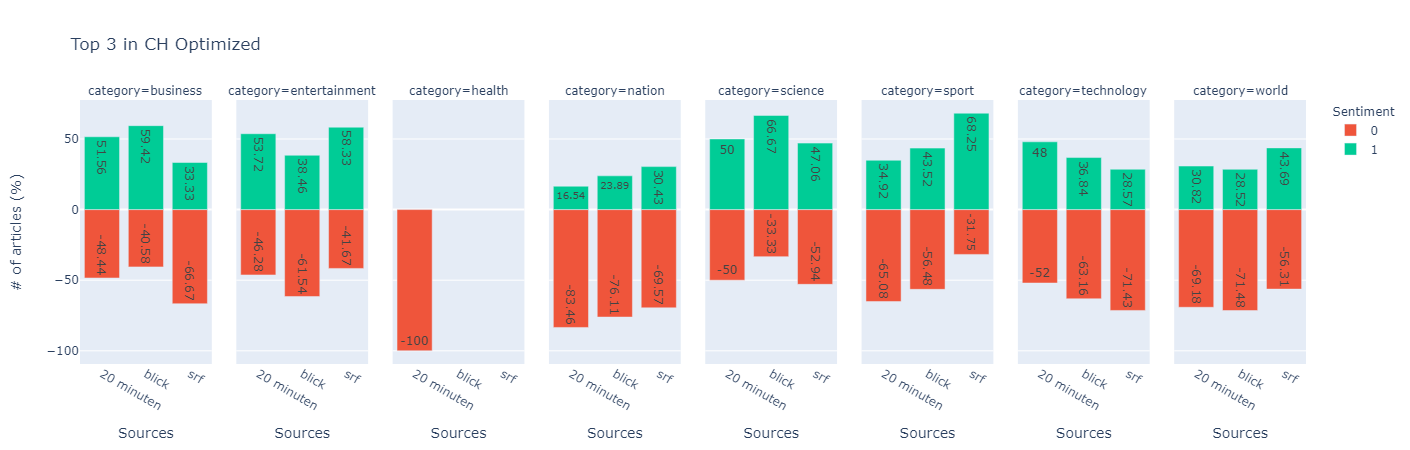
\includegraphics[width=1.25\textwidth,center]{images/top32.png}
\caption{Top 3 newspaper improvement}
\label{fig:fig_improvement}
\end{figure}

In detail, "20 Minuten" is the newspaper with the highest negativity in several categories.
"Health" category only has 2 articles, so it is not one to be overly considered.
While the category with the most negativity is once again "nation".
This is a high negativity, considering that this newspaper is free and can be found everywhere.

\subsubsection{Spider plot per category of a single newspaper} 
The \gls{plot} in Figure~\ref{fig:fig_spider} gives an idea of the area that each newspaper covers based on the categories. I then created a function to be able to easily \gls{plot} a list of given newspapers, without having to write everything by hand.

\begin{figure}[H]
\centering
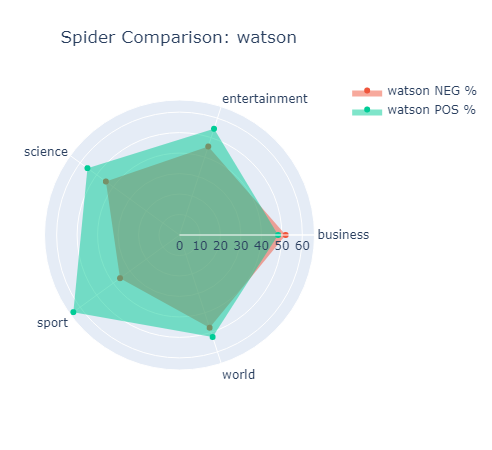
\includegraphics[width=0.65\textwidth]{images/wats.png}
\caption{Newspaper spider}
\label{fig:fig_spider}
\end{figure}
\FloatBarrier
Each point on the \gls{plot} equals the percentage of positivity (in green) or negativity (in red) of a given category. By connecting all the points I define the area of positivity and negativity of each newspaper.

Not just negative newspaper, fortunately. Watson is the newspaper that expresses articles with the most positivity. In fact, in almost every category it has a higher percentage of positivity than negativity.


\subsubsection{Plot in time per newspaper} 
The \gls{plot} in Figure~\ref{fig:fig_timenews} shows the trend of a newspaper over time.
The top 3 newspapers were chosen because they are the ones that influence the most in the Swiss territory.
The time span is from May 1, 2021 until today.

\begin{figure}[H]
 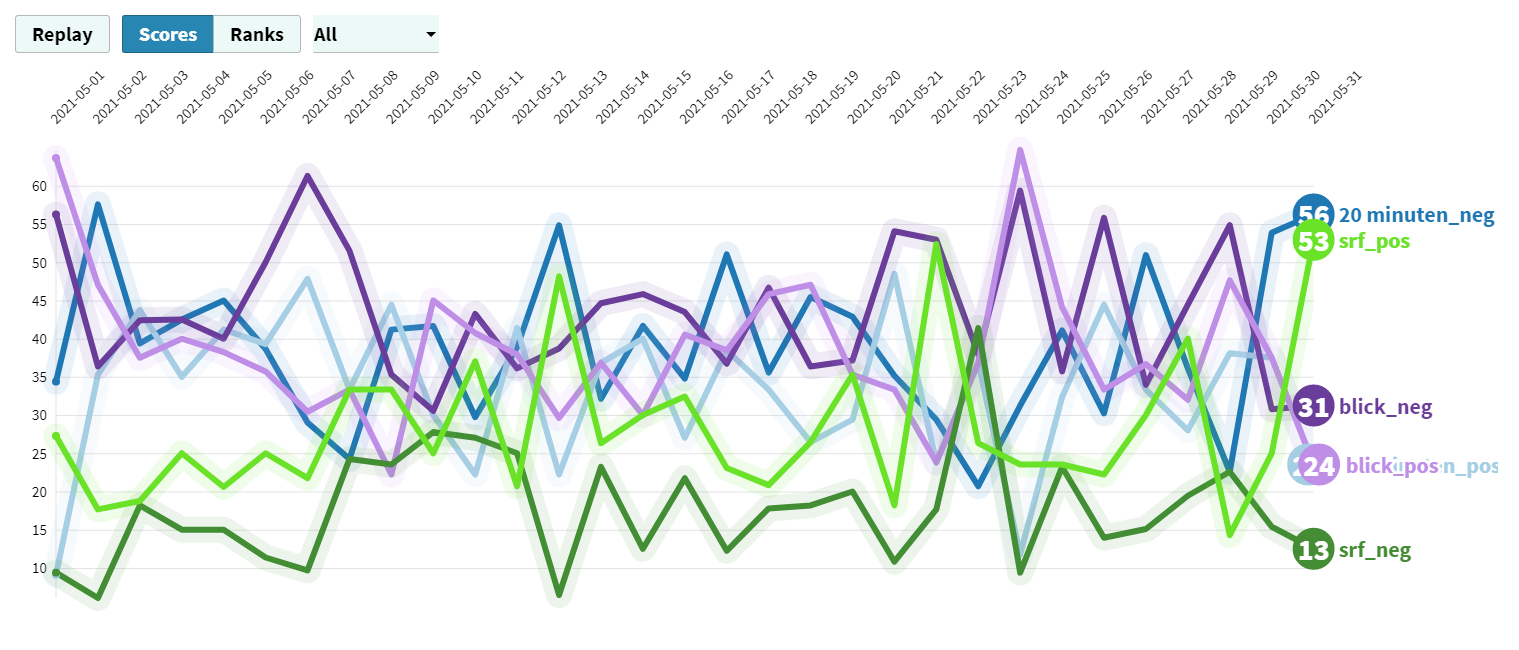
\includegraphics[width=1.2\textwidth,center]{images/POSneg.png}
\caption{Newspaper in time}
\label{fig:fig_timenews}
\end{figure}
\FloatBarrier

The \gls{plot} presents on the x-axis the time range, and on the y-axis the percentage of positivity or negativity that a paper had over a single day.
Each newspaper then is divided into two colors in order to distinguish the positive and negative sentiment. For the division of colors I took into consideration per newspaper two similar colors. The darker color of the two represents negative sentiment, the lighter color represents positive sentiment.

It can be seen that:
\begin{itemize}
    \item "blick" has the highest peaks of negative values over time, often exceeding 50\%.
    \item "srf" remains fairly constant, with more positive articles,
    \item "20 minuten" as well as "blick" have a tendency to be more negative over time.
\end{itemize}


\subsubsection{Plot in time per category}
The \gls{plot} in Figure~\ref{fig:fig_cattime} is an interesting \gls{plot} because it shows the trend over time as events occur.

\begin{figure}[H]
 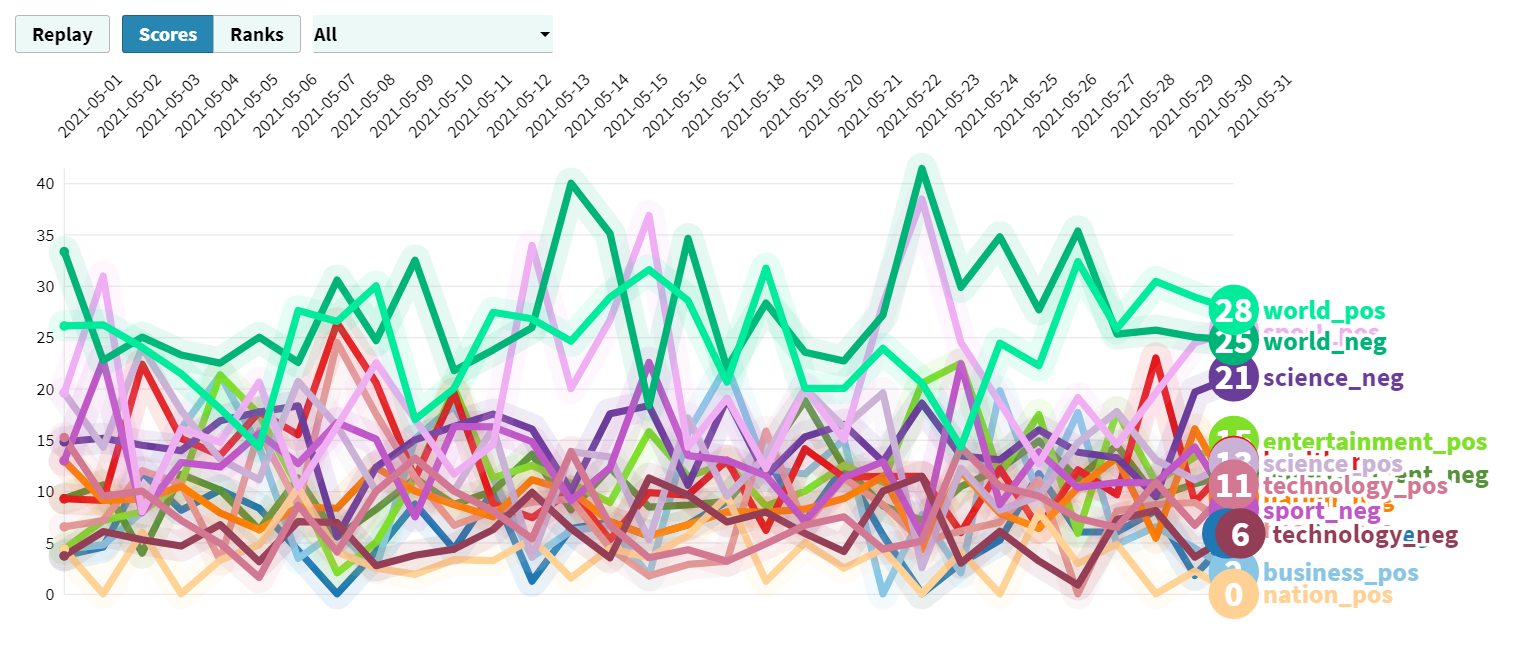
\includegraphics[width=1.2\textwidth,center]{images/CategoryPOSneg.png}
\caption{Newspaper in time}
\label{fig:fig_timenews}
\end{figure}
\FloatBarrier

The \gls{plot} presents on the x-axis the time range, and on the y-axis the percentage of positivity or negativity that a category had over a single day.
Each category is divided into two colors in order to distinguish positive and negative feeling. For the subdivision of colors I have taken into consideration per category two similar colors. The lighter color of the two represents positive sentiment, the darker color represents negative sentiment.

Categories are:
\begin{itemize}
    \item business pos(light blue)/neg(blue)
    \item entertainment pos(light green)/neg(dark green)
    \item health pos(light red)/neg(red)
    \item nation pos(light orange)/neg(orange)
    \item science pos(violet)/neg(lila)
    \item sport pos(pink)/neg(fuchsia)
    \item technology pos(light brown)/neg(brown)
    \item world pos(aqua green)/neg(dark aqua green)
\end{itemize}

The category that immediately jumps out is the negative "world" one.
Recently, negative events have occurred between Palestine and Israel. As of May 17, the category world has had a boost in negative sentiment. On the 23rd of May there was a cableway accident in Italy in which several people died, for this reason also on that day the category "world" had a peak.

It would have been nice to see the performance of the newspapers before and during the pandemic. 
Being the end of May, maybe I am lucky enough to see the change in direction of the pandemic, like last year in fact in summer it has less effect. Taking into consideration also the vaccination campaign, I speculate that it will be possible to see an improvement in the situation in almost all categories of newspaper. 